\documentclass[12pt,answers]{exam}

\usepackage{amsmath,amsfonts,amssymb,mathtools,physics,commath}
\usepackage{todonotes}
\usepackage{float}
\usepackage{multicol}
\usepackage{polynom}
\usepackage{siunitx}

\newcommand{\inv}{^{-1}}

\pagestyle{headandfoot}
\firstpageheadrule
\runningheadrule
\firstpageheader{Math 221}{Final Exam|Solutions, Page \thepage\ of \numpages}{May 13, 2020}
\runningheader{Math 221}{Final Exam|Solutions, Page \thepage\ of \numpages}{May 13, 2020}
\runningfooter{}{}{}

\begin{document}
% \maketitle
\begin{questions}

\question[10]
Evaluate the following integral.
\\
$\displaystyle \int x \tan\inv(x) \dif x$, where $\tan\inv(x)$ is the inverse tangent function.
\begin{solution}
    \[
    \begin{array}{ccc}
        & D & I \\ 
        + & \tan\inv(x) & x \\ 
        - & \dfrac{1}{x^2+1} & \dfrac{x^2}{2}
    \end{array}
    \]
    \begin{align*}
        \int x \tan\inv(x) \dif x
        &= \frac12 x^2 \tan\inv(x) - \frac 12 \int \frac{x^2}{x^2+1} \dif x \\ 
        &= \frac 12 x^2 \tan\inv(x) - \frac 12 \int \left(1- \frac{1}{x^2+1}\right) \dif x \\ 
        &= \boxed{\frac 12 x^2 \tan\inv(x) - \frac 12 x + \frac 12 \tan\inv x +C }
    \end{align*}
\end{solution}

\question[12]
Evaluate the following integral.
$\displaystyle \int \frac{x^2 \dif x}{\sqrt{1-x^2}}$
\begin{solution}
    $x = \sin \theta$, $\dif x = \cos \theta \dif \theta$
    \begin{multicols}{2}
    \begin{align*}
        \int \frac{x^2 \dif x}{\sqrt{1-x^2}}
        &= \int \frac{\sin^2 \theta \cos \theta \dif \theta}{\sqrt{1-\sin^2 \theta}} \\
        &= \int \sin^2 \theta \dif \theta \\
        &= - \frac{\sin \theta \cos \theta}{2} + \frac12 \int 1 \dif \theta \\
        &= -\frac12 \sin\theta\cos\theta + \frac12 \theta \\
        &= \boxed{- \frac 12 x \sqrt{1-x^2} + \frac12 \sin\inv x + C}
    \end{align*}
    \begin{figure}[H]
        \centering
        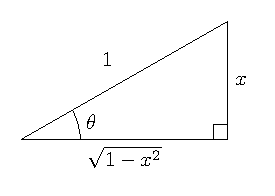
\includegraphics{graphics/2020-spring-final-2.pdf}
    \end{figure}
\end{multicols}
\end{solution}

\newpage
\question[10]
Evaluate the integral.
$\displaystyle \int \frac{e^{2x}}{5+e^{2x}} \dif x$
\begin{solution}
    $u = e^{2x}$, $\dif u = 2e^{2x} \dif x$
    so
    \begin{align*}
        \int \frac{e^{2x}}{5+e^{2x}} \dif x
        &= \frac 12 \int \frac{1}{5+u} \dif u \\ 
        &= \frac 12 \ln|u+5| \\
        &= \boxed{\frac 12 \ln(e^{2x} + 5) + C}
    \end{align*}
\end{solution}

\question[12]
Evaluate the integral.
$\displaystyle \int \frac{3x^2+8}{x^3+4x} \dif x$
\begin{solution}
    \[
        \frac{3x^2+8}{x(x^2+4)} = \frac{2}{x} + \frac{x}{x^2+4}
    \]
    \begin{align*}
        \int \frac{3x^2+8}{x^3+4x} \dif x
        &= \int \left( \frac2x + \frac{x}{x^2 + 4}\right) \dif x \\ 
        &= \boxed{2 \ln|x| + \frac12 \ln(x^2+4) + C}
    \end{align*}
\end{solution}

\question[10] 
Evaluate the improper integral or show that it diverges. Use limit notation.
$\displaystyle \int_1^5 \frac{\dif x}{\sqrt{x-1}}$
\begin{solution}
    \begin{align*}
        \lim_{b\to1^-} \int_b^5 \frac{\dif x}{\sqrt{x-1}}
        &= 
        \lim_{b\to1^-} \left[ \eval{2\sqrt{x-1}}_b^5 \right]\\
        &= 
        \lim_{b\to1^-} \left( 2\sqrt{4} - 2\sqrt{b-1}\right)
        = 4 - 0 = \boxed{4}
    \end{align*}
\end{solution}

\newpage
\question[8]
Explain why the following series converges, and then evaluate it.
\\
$\displaystyle \sum_{n=1}^\infty \frac2\pi \left(-\frac\pi4\right)^n$
\begin{solution}
    This is a geometric series with $a = \frac 2\pi (-\frac\pi4) = -\frac12$ and $r= -\frac\pi4$. It converges since $\abs{-\frac\pi4} < 1$.
    The series converges to 
    \[
        \frac{a}{1-r} 
        = \frac{-\frac12}{1-(-\frac\pi4)} 
        = \frac{-\frac12}{\frac{\pi+4}{4}}
        = \boxed{\frac{-2}{\pi+4}}
    \]
\end{solution}

\question
Let $R$ be the region trapped between $y=x$ and $y=x^2$, with $0 \le x \le 1$.
\begin{parts}
    \part[6]
    Find the area of the region $R$.
\begin{solution}
    \begin{align*}
        \int_0^1 (x - x^2) \dif x
        = \left[\frac12 x^2 - \frac13 x^3 \right]_0^1
        = \frac12 - \frac 13 - 0 
        = \boxed{\frac 16}
    \end{align*}
\end{solution}
    \part[10]
    Find $\overline y$, the $y$ coordinate of the centroid of $R$. (Do not calculate $\overline x$.)
\begin{solution}
    \begin{align*}
        M_x &= \frac12 \int_0^1 \left(x^2 - (x^2)^2\right) \dif x
        = \frac 12 \left[ \frac13 x^3 - \frac 15 x^5 \right]_0^1 
        = \frac{1}{15}  \\
        \overline y 
        &= \frac{M_x}{m}
        = \frac{1}{15} \cdot 6 = \boxed{\frac{2}{5}}
    \end{align*}
\end{solution}
\end{parts}

\newpage
\question
Let $\displaystyle S = \sum_{n=1}^\infty \frac{(-1)^{n+1}}{2n+1}$.
\begin{parts}
    \part[4]
    Explain why the series converges.
    \begin{solution}
        The sequence $b_n = \frac{1}{2n+1}$ is decreasing and has $\lim_{n\to\infty} b_n = 0$, so by 
        Alternating Series Test, the series converges.
    \end{solution}
    \part[4]
    How many terms are required to approximate $S$ with an error less than 0.01?
    \begin{solution}
        The error of an alternating series is bounded by the next term:
        \[
        |S - S_N| \le b_{N+1}.
        \]
        So to ensure the error bounds, we enforce
        \begin{align*}
            \frac{1}{2(N+1)+1} \le 0.01 = \frac{1}{100}
            &\implies 100 \le 2(N+1)+1 \\
            &\implies \frac{99}{2} - 1 \le N \\
            &\implies N \ge \frac{97}{2} = 48.5
        \end{align*}
        Thus $N = 49$ suffices.
    \end{solution}
\end{parts}

\newpage
\question[12]
Find the interval of convergence of the power series $\displaystyle \sum_{n=1}^\infty \frac{(x-2)^n}{n \cdot 4^n}$.
(Make clear the status of any end points.)
\begin{solution}
    \begin{align*}
    \lim_{n\to\infty} \left| \frac{(x-2)^{n+1}}{(n+1) \cdot 4^{n+1}} \cdot \frac{n\cdot 4^n}{(x-2)^n}\right|
    = \lim_{n\to\infty} \left| \frac{x-2}{4} \cdot \frac{n}{n+1} \right|
    &= \frac14 |x-2| \cdot 1 < 1 \\ 
    &\implies |x-2| < 4 \\
    &\implies -2 < x < 6
    \end{align*}
    At $x = 6$:
    \[
        \sum_{n=1}^\infty \frac{4^n}{n \cdot 4^n} 
        = \sum_{n=1}^\infty \frac{1}{n} \text{ diverges (harmonic series)}
    \]
    At $x = -2$:
    \[
        \sum_{n=1}^\infty \frac{(-4)^n}{n \cdot 4^n} = \sum_{n=1}^\infty \frac{(-1)^n}{n} \text{ converges (alternating harmonic series)}
    \]
    Thus the interval of convergence is $\boxed{\intco{-2, 6}}$
\end{solution}

\question[12]
Solve the initial value problem, $(1+t^2) \dod{y}{t} = 2t e^y$, $y(0) = 1$. 
Express your final answer in the form $y = f(t)$.
\begin{solution}
    \begin{align*}
        (1+t^2) \dod{y}{t} &= 2t e^y \\ 
        \int e^{-y} \dif y &= \int \frac{2t}{1+t^2} \dif t \\ 
        -e^{-y} &= \ln(1+t^2) + C \\ 
        y &= -\ln(-\ln(1+t^2) - C) \\ 
        y(0) &= -\ln(-\ln(1) - C) = 1 \\ 
        &\implies \ln(-C) = -1 \\ 
        &\implies C = -e^{-1} \\ 
        \implies \Aboxed{y(t) &= -\ln(-\ln(1+t^2) + e^{-1})}
    \end{align*}
\end{solution}

\question
Determine whether the following series converge or diverge.
State clearly which test you are using and implement the test as clearly as you can.
The answer is worth 2 points and the work you show 4 points.
\begin{parts}
    \part[6]
    $\displaystyle \sum_{n=3}^\infty \frac{\sqrt n}{n^2+1}$
    \begin{solution}
        Comparing with the series $\displaystyle \sum \frac{1}{n^{3/2}}$:
        \[
            \lim_{n\to\infty} \frac{\frac{\sqrt n}{n^2+1}}{\frac{1}{n^{3/2}}} 
            = \lim_{n\to\infty} \frac{n^2}{n^2+1}
            = 1
        \]
        Since $\sum \frac{1}{n^{3/2}}$ converges ($p$-series test with $p = 3/2 > 1$), by Limit Comparison Test, the series \fbox{converges}
        \\
        \textit{Remark:} Direct Comparison Test can also be used, since $\displaystyle \sum \dfrac{\sqrt{n}}{n^2+1} < \sum \dfrac{\sqrt{n}}{n^2} = \sum \dfrac{1}{n^{3/2}}$
    \end{solution}
    \part[6]
    $\displaystyle \sum_{n=2}^\infty \frac{\cos(1/n)}{2 + \sin(1/n)}$
    \begin{solution}
        Since 
        \[
            \lim_{n\to\infty} \frac{\cos(1/n)}{2+\sin(1/n)} = \frac{1}{2} \ne 0
        \]
        this series \fbox{diverges} by Divergence Test.
    \end{solution}
\end{parts}

\question[6]
Determine whether the following series converges or diverges.
State clearly which test you are using and implement the test as clearly as you can.
The answer is worth 2 points and the work you show 4 points.
\\
$\displaystyle \sum_{n=1}^\infty \left(\frac{2n^2-3}{n^2+7n}\right)^n$
\begin{solution}
    Using root test:
    \[
        \lim_{n\to\infty} \sqrt[n]{\left(\frac{2n^2-3}{n^2+7n}\right)^n}
        = \lim_{n\to\infty} \frac{2n^2-3}{n^2+7n} = 2 > 1
    \]
    By root test, the series \fbox{diverges}
\end{solution}

\newpage
\question[12]
Find the third degree Taylor polynomial $T_3(x)$ for the function $f(x) = \cos x$ centered at $x = \pi/2$.
\begin{solution}
    \begin{align*}
        f(x) &= \cos x 
        &f(\pi/2) &= 0 \\ 
        f'(x) &= -\sin x 
        &f'(\pi/2) &= -1 \\ 
        f''(x) &= -\cos x 
        &f''(\pi/2) &= 0 \\ 
        f'''(x) &= \sin x 
        &f'''(\pi/2) &= 1 \\ 
    \end{align*}
    \begin{align*}
        T_3(x) 
        &= 0 + -1\left(x-\frac\pi2\right) + \frac{0}{2!} \left(x-\frac\pi2\right)^2 + \frac{1}{3!}\left(x-\frac\pi2\right)^3 \\
        &= \boxed{-\left(x-\frac\pi2\right) + \frac16 \left(x-\frac\pi2\right)^3}
    \end{align*}
\end{solution}

\question[8]
Use the series expansions for $e^x$ and $(1+x)^n$ on the cover page to find the terms up to $x^4$ for the Maclaurin series of $e^{x^2} \sqrt{1+x^2}$
\begin{solution}
    \begin{align*}
        e^{x^2} 
        &= \sum_{n=0}^\infty \frac{x^{2n}}{n!} = 1 + x^2 + \frac 12 x^4 + \frac16 x^6 + \cdots \\ 
        (1+x^2)^{1/2} 
        &= 1 + \frac12 x^2 + \frac{\frac12 (-\frac12)}{2}x^4 + \cdots \\
        &= 1 + \frac12 x^2 - \frac18 x^4 + \cdots \\
        e^{x^2} \sqrt{1+x^2} 
        &= \left(1 + \frac12 x^2 - \frac 18 x^4 + \cdots \right)
        + \left( x^2 + \frac12 x^4 + \cdots \right)
        + \left(\frac12 x^4 + \cdots \right) + \cdots \\ 
        &= \boxed{1 + \frac32 x^2 + \frac78 x^4} + \cdots
    \end{align*}
\end{solution}

\newpage
\question
\begin{parts}
    \part[5]
    Use an appropriate series for the cover sheet to find the Maclaurin series for $\dfrac{1}{1+x^5}$
    \begin{solution}
        \begin{align*}
            \frac{1}{1-x} &= \sum_{n=0}^\infty x^n \\ 
            \frac{1}{1-(-x^5)} &= \sum_{n=0}^\infty (-x^5)^n \\ 
            \frac{1}{1+ x^5} &= \boxed{\sum_{n=0}^\infty (-1)^n x^{5n}}
        \end{align*}
    \end{solution}
    \part[3]
    Use your answer to part (a) to find the Maclaurin series for $\dfrac{x^3}{1+x^5}$
    \begin{solution}
        \[
            \frac{x^3}{1+x^5} = x^3 \sum_{n=0}^\infty(-1)^n x^{5n} = \boxed{\sum_{n=0}^\infty (-1)^n x^{5n+3}}
        \]
    \end{solution}
    \part[7]
    Use your answer to part (a) to evaluate the following integral, expressing your final answer as an infinite series.
    $\displaystyle\int_0^1 \frac{\dif x}{1+x^5}$
    \begin{solution}
        \begin{align*}
            \int_0^1 \frac{\dif x}{1+x^5} 
            &= \int_0^1 \sum_{n=0}^\infty (-1)^n x^{5n} \\
            &= \sum_{n=0}^\infty \left[\frac{(-1)^n}{5n+1} x^{5n+1}\right]_0^1 \\ 
            &= \boxed{\sum_{n=0}^\infty \frac{(-1)^n}{5n+1}}
        \end{align*}
    \end{solution}
\end{parts}

\newpage
\question Consider the curve with parameric equations $x = t^2 + 1$, $y = 2t^3$, $t \ge 0$.
\begin{parts}
    \part[4]
    Find the slope of the curve at a general value $t$.
    \begin{solution}
        \begin{align*}
            \dod{y}{x} = \frac{\dod{y}{t}}{\dod{x}{t}} = 
            \frac{6t^2}{2t} = \boxed{3t}
        \end{align*}
    \end{solution}
    \part[4]
    Find the equation of the tangent line to the curve at $t = 1$.
    \begin{solution}
        \begin{align*}
        m &= \eval{\dod{y}{x}}_{t=1} = 3 \\ 
        x(1) &= 2 \\ 
        y(1) &= 2 \\
        \Aboxed{y - 2 &= 3(x-2)}
        \end{align*}
    \end{solution}
    \part[4] 
    Convert the equation to a rectangular equation in $x,y$.
    \begin{solution}
        \begin{align*}
            x &= t^2 + 1 \implies t^2 = x - 1\\
            y &= 2t^3 = \boxed{2 (x-1)^{3/2}}
        \end{align*}
    \end{solution}
\end{parts}

\newpage
\question[8]
Find the length of the curve $x = t^2 + 1$, $y = 2t^3$, $0 \le t \le 1$.
\begin{solution}
    \begin{align*}
        L = \int_0^1 \sqrt{x'(t)^2 + y'(t)^2} \dif t
        &= \int_0^1 \sqrt{(2t)^2 + (6t^2)^2} \dif t \\ 
        &= \int_0^1 \sqrt{4t^2 + 36 t^4} \dif t \\ 
        &= \int_0^1 \sqrt{4t^2(1+9t^2)}  \dif t \\ 
        &= \int_0^1 2t \sqrt{1+9t^2} \dif t  & (u = 1+9t^2; \dif u = 18t \dif t)\\ 
        &= \frac 19 \int_1^{10} \sqrt u \dif u \\ 
        &= \frac19 \cdot \frac 23 \left[ u^{3/2}\right]_1^{10} \\ 
        &= \boxed{\frac{2}{27} (10^{3/2} - 1)}
    \end{align*}
\end{solution}

\newpage
\question
\begin{parts}
    \part[6]
    Convert the polar equation $r = 2\sin \theta + 4 \cos \theta$, to a rectangular equation in $x, y$.
\begin{solution}
    \begin{gather*}
        r^2 = 2 r\sin \theta + 4 r\cos \theta \\ 
        x^2 + y^2 = 2 y + 4x  \\ 
        x^2 -4x + 4 + y^2 - 2y + 1 = 4 + 1 \\ 
        \boxed{(x-2)^2 + (y-1)^2 = (\sqrt 5)^2}
    \end{gather*}
    (Circle centered at $(2, 1)$ with radius $\sqrt 5$)
\end{solution}
    \part[5]
    Sketch the graph of the polar equation in part (a) with $0 \le \theta \le \frac\pi2$. (Note: $\sqrt 2 \approx 1.4$, $\sqrt 3 \approx 1.7$, $\sqrt 5 \approx 2.2$.)
\begin{solution}
    \begin{multicols}{2}
    \begin{tabular}{c|l}
        $\theta$ & $r = 2 \sin \theta + 4 \cos \theta$ \\ 
        \hline
        0 & 0 + 4 = 4 \\ 
        $\pi/4$ & $2 \cdot \frac{\sqrt 2}{2} + 4 \cdot \frac{\sqrt 2}{2} = 3 \sqrt 2 \approx 4.2$ \\ 
        $\pi/2$ & 2 + 0 = 2 
    \end{tabular}    
    \begin{figure}[H]
        \centering
        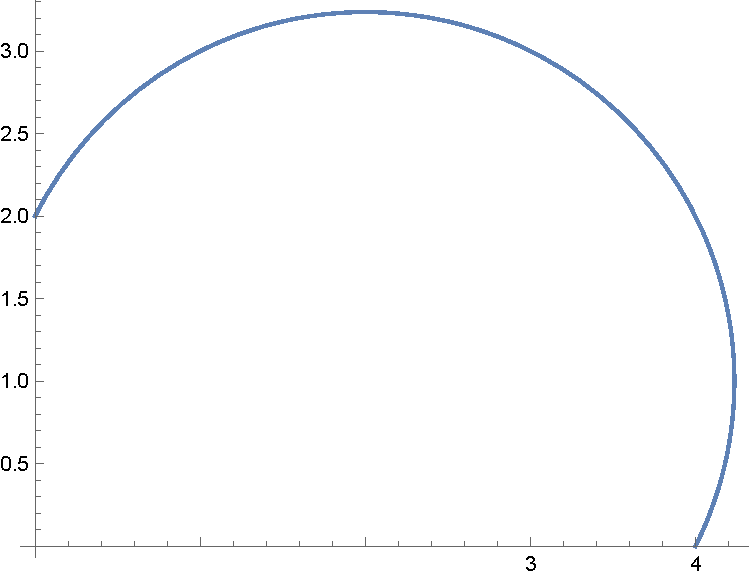
\includegraphics[width=.8\linewidth]{graphics/2020-spring-final-18b.pdf}
    \end{figure}
    \end{multicols}
\end{solution}
\end{parts}

% \newpage
\question[6]
Find the slope of the polar curve $r = 2\sin\theta + 4\cos\theta$ at $\theta = \pi/2$.
\begin{solution}
    \begin{align*}
        x &= r \cos \theta = (2\sin \theta \cos \theta + 4\cos^2 \theta) \\ 
        y &= r \sin \theta = (2\sin^2 \theta + 4\sin\theta \cos \theta)
    \end{align*}
    \begin{align*}
        \dod{y}{x} 
        = \frac{\dod{y}{\theta}}{\dod{x}{\theta}}
        &= \frac{2 \cdot 2 \sin\theta \cos \theta + 4 \sin\theta (-\sin \theta) + 4 \cos \theta \cos \theta }{2 \sin\theta(-\sin \theta) + 2 \cos^2\theta + 8 \cos \theta (-\sin\theta)} \\ 
        m = \eval{\dod{y}{x}}_{\theta=\pi/2} 
        &= \frac{4 \cdot 0 - 4 + 0}{-2 + 0 + 0} 
        = \frac{-4}{-2} = \boxed{2}
    \end{align*}
\end{solution}

\end{questions}
\end{document}